%% Based on a TeXnicCenter-Template by Gyorgy SZEIDL.
%%%%%%%%%%%%%%%%%%%%%%%%%%%%%%%%%%%%%%%%%%%%%%%%%%%%%%%%%%%%%

%------------------------------------------------------------
%
\documentclass[titlepage]{article}%
%Options -- Point size:  10pt (default), 11pt, 12pt
%        -- Paper size:  letterpaper (default), a4paper, a5paper, b5paper
%                        legalpaper, executivepaper
%        -- Orientation  (portrait is the default)
%                        landscape
%        -- Print size:  oneside (default), twoside
%        -- Quality      final(default), draft
%        -- Title page   notitlepage, titlepage(default)
%        -- Columns      onecolumn(default), twocolumn
%        -- Equation numbering (equation numbers on the right is the default)
%                        leqno
%        -- Displayed equations (centered is the default)
%                        fleqn (equations start at the same distance from the right side)
%        -- Open bibliography style (closed is the default)
%                        openbib
% For instance the command
%           \documentclass[a4paper,12pt,leqno]{article}
% ensures that the paper size is a4, the fonts are typeset at the size 12p
% and the equation numbers are on the left side
%
\usepackage{amsmath}%
\usepackage{amsfonts}%
\usepackage{amssymb}%
\usepackage{graphicx}
%-------------------------------------------
\renewcommand\abstractname{Summary}
\newtheorem{theorem}{Theorem}
\newtheorem{acknowledgement}[theorem]{Acknowledgement}
\newtheorem{algorithm}[theorem]{Algorithm}
\newtheorem{axiom}[theorem]{Axiom}
\newtheorem{case}[theorem]{Case}
\newtheorem{claim}[theorem]{Claim}
\newtheorem{conclusion}[theorem]{Conclusion}
\newtheorem{condition}[theorem]{Condition}
\newtheorem{conjecture}[theorem]{Conjecture}
\newtheorem{corollary}[theorem]{Corollary}
\newtheorem{criterion}[theorem]{Criterion}
\newtheorem{definition}[theorem]{Definition}
\newtheorem{example}[theorem]{Example}
\newtheorem{exercise}[theorem]{Exercise}
\newtheorem{lemma}[theorem]{Lemma}
\newtheorem{notation}[theorem]{Notation}
\newtheorem{problem}[theorem]{Problem}
\newtheorem{proposition}[theorem]{Proposition}
\newtheorem{remark}[theorem]{Remark}
\newtheorem{solution}[theorem]{Solution}
\newtheorem{summary}[theorem]{Summary}
\newenvironment{proof}[1][Proof]{\textbf{#1.} }{\ \rule{0.5em}{0.5em}}

\begin{document}

%======================================== Title Page ==================================
\pagestyle{empty}
\begin{center}

\includegraphics[scale=0.3]{TU-Signet.png}
\vspace{1cm}
{\Large \\Project for the subject Modelling and Simulation\\}
\vspace{1cm} 
{\huge Production Chain in a Bakery - DEVS\\}	%===== Title of your dissertation
\vspace{5cm}
{Submitted To:\\}
\vspace{0.3cm}
{Univ.-Lecturer\\}
{Franz Josef Preyser\\}
{Institut für Analysis und Scientific Computing\\}
{Faculty of Informatics\\}

\vspace{2cm}
{Submitted By:\\}
\vspace{0.3cm}
{Jawad Haider KAZMI (1328102), \\ Ishtiaque AHMAD (1229645), \\ Ikram ULLAH (1329824) \\}						%===== Your Name here
{Matriculation No: xxxxxxxxx\\} 	%===== Your Matriculation number in place of xxxxxxxxxx
\vspace{3cm}
March, 2015
\end{center}
%========================================Table of Contents=====================================

\newpage
\tableofcontents
\newpage

%========================================Abstract===============================================
\begin{abstract}

The task of this project is to implement an simple DEVS-Model of a baking-oven with a DEVS-able simulation. The implemented model is described as follows;
At a certain point in time, portion of a paste with the attributes mass m and (up to now accumulated) costs K arrives at the Oven. If the oven is currently in the waiting - state (i.e. process-phase p=0), then the paste attributes a stored in the oven state variables m and K and the process-phase p is incremented (i.e. p:=1). This is all done by the external transition function δext . If process phase p=1, the paste is baking for the duration T1. That is, the next event to be triggered is an internal event, which happened exactly T1 after the previous external event, where the paste arrived. This internal event leads to the execution of  δint , which adds the costs K2 that arose from the baking phase to the accumulated costs K and increments the process phase p to p=2. p=2 means unloading-phase. The duration of the unloading phase is T2. Therefore after T2 the next internal event is triggered which again results in the execution of δint. But this time , there is an output to be generated as well. So right before δint is executed, the output function lambda computed an "output-message". In our case, the output represents the baked bread, which again has the attributes mass m and costs K. the mass stays the same, so m will be set to the value stored as state variable m. Since the unloading phase also produce costs, the costs K will be set to the value stored as state variable K plus the costs K2 that arose in phase 2. After the output has been calculated, the internal transition function sets the state variables m and K to 0 also resets the process phase p to 0, meaning "waiting for the next paste to arrive." 
\vspace{1cm}

\noindent {\large \bfseries{Keywords:~}} 
\end{abstract}


%======================================== Main Text =====================================
\newpage
\setcounter{page}{1}
\pagestyle{plain}

\section{Task-1 DEVS-Model  for Baking Oven}

\subsection{Description}

The task of this project is to implement an simple DEVS-Model of a baking-oven with a DEVS-able simulation. The implemented model is described as follows;
At a certain point in time, portion of a paste with the attributes mass m and (up to now accumulated) costs K arrives at the Oven. If the oven is currently in the waiting - state (i.e. process-phase p=0), then the paste attributes a stored in the oven state variables m and K and the process-phase p is incremented (i.e. p:=1). This is all done by the external transition function δext . If process phase p=1, the paste is baking for the duration T1. That is, the next event to be triggered is an internal event, which happened exactly T1 after the previous external event, where the paste arrived. This internal event leads to the execution of  δint , which adds the costs K2 that arose from the baking phase to the accumulated costs K and increments the process phase p to p=2. p=2 means unloading-phase. The duration of the unloading phase is T2. Therefore after T2 the next internal event is triggered which again results in the execution of δint. But this time , there is an output to be generated as well. So right before δint is executed, the output function lambda computed an "output-message". In our case, the output represents the baked bread, which again has the attributes mass m and costs K. the mass stays the same, so m will be set to the value stored as state variable m. Since the unloading phase also produce costs, the costs K will be set to the value stored as state variable K plus the costs K2 that arose in phase 2. After the output has been calculated, the internal transition function sets the state variables m and K to 0 also resets the process phase p to 0, meaning "waiting for the next paste to arrive." 
\subsection{Paste arrive scenario}

We have implemented a Queue to handle the situation when the process phase p is not zero and a paste arrives. If p is not zero and a paste is ready , it is added to the queue. After the execution of internal function and completion of phase 2 , queue is checked , if it is not empty then paste is picked from the queue on the basis of first in first out (FIFO). 




\section{Task-2 : Implementation of Baking Oven Model in PowerDEVS}


%to develop a co-simulation tool for combined power system (physical), communication and control (cyber) simulation and then, uses it to evaluation and quantify reliability of the simulated system. 
%Unavailability of such insight could results in a poorly designed systems which could results in a possible economical and social loss.


\section{Task-3 : Documentation}
\subsection{DEVS-Formalism}

DEVS is an acronym for Discrete Event System . This is a formalism that was first introduced by Bernard Zeigler. It is used for the description of discrete event system.  A DEVS model has input events which are processed to produce output events(results). Output events are influenced by  input events and  initial conditions of the model.Figure  \ref{atomic_model} shows a basic structure of an atomic model.  An Atomic DEVS model has the following formulation;

Where

X 		: set of input event values, i.e., the set of all possible values that
		an input event can have
Y 		: set of possible output event values
S 		: set of possible states values
δ ext 	: External state transition function
δ int 	: Internal state transition function
ta	  	: Time advance  Function

\begin{figure}[h!]
  \centering
    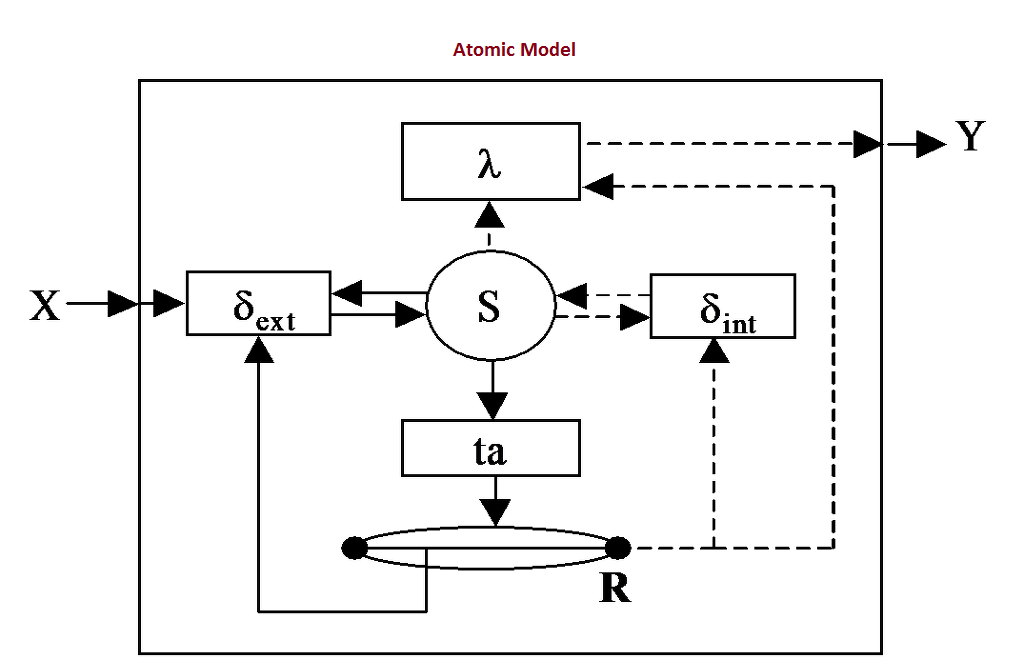
\includegraphics[width=0.5\textwidth]{Fig1.png}
    \caption{Atomic Model}
    \label{atomic_model}
\end{figure}


\subsection{DEVS-Model for Baking Oven}
\subsection{Simulation Tool Experiences}


PowerDEVS is a general purpose software tool for DEVS modeling and simulation oriented to the simulation of hybrid systems. It allows defining atomic DEVS models in C++ language that can be then graphically coupled in hierarchical block diagrams to create more complex systems. The environment automatically translates the graphically coupled models into a C++ code which executes the simulation \cite{BK11}.
One of the features of PowerDEVS is the synchronization of simulation in real time operating system with real time clock, which allows the design and implementation of synchronous and asynchronous digital controller. PowerDEVS is also efficient tool for real time simulation of physical systems when combined with continuous system simulation library. The interconnection of PowerDEVS with the numerical package Scilab is another attractive feature of PowerDEVS. The variables and functions in the workspace of Scilab can be used by PowerDEVS, and Scilab can process and analyze the result data sent from PowerDEVS.
PowerDEVS is composed of various independent programs: 



\subsubsection{The Model Editor} 
It is the main program of PowerDEVS which provides graphical interface for building and managing models and library, launching simulation, editing elementary blocks up to atomic model definitions and link with other application of PowerDEVS. 
 
 
 \begin{figure}[h!]
  \centering
    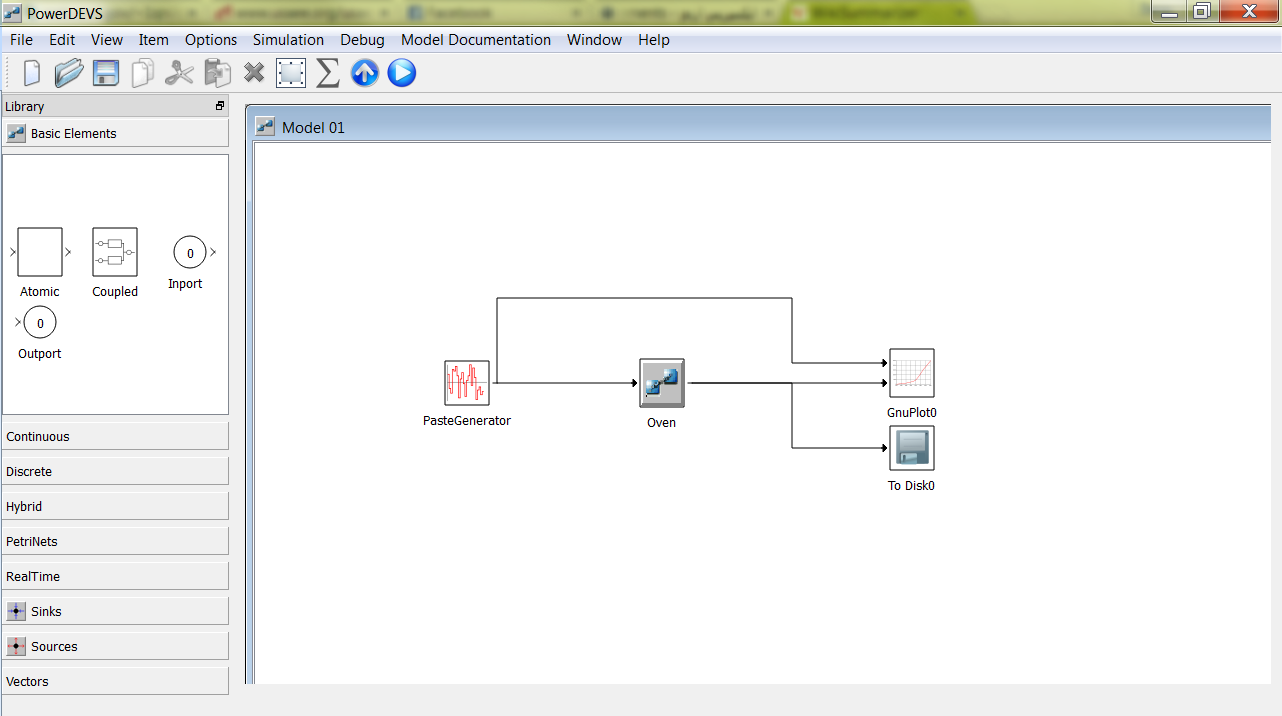
\includegraphics[width=0.5\textwidth]{Fig2.png}
    \caption{Model Editor main window}
    \label{model_edt}
\end{figure}
 
The Model Editor main window shown in Figure \ref{model_edt} is used to create and open models and libraries. At the left the list if libraries can be selected and blocks can be dragged from the libraries to the models. The selected library is active and the blocks are visible under the selected library. Models and libraries can be edited in a model window with the open and new model commands. The model window in Figure \ref{model_win} showing model consist of with four sub models.


 \begin{figure}[h!]
  \centering
    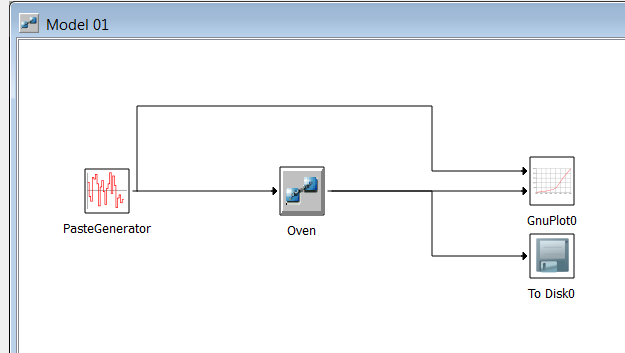
\includegraphics[width=0.5\textwidth]{Fig3.png}
    \caption{Model Window}
    \label{model_win}
\end{figure}

In the model windows the typical graphical edition facilities are provided so that blocks can be copied, resized, rotated, etc. while the connections between different ports can be directly drawn. The edit menu or using the right button the features of each blocks either a coupled or an atomic model can be edited. The block edition window shown in Figure \ref{Block_win} is used to configure the graphic appearance of the block and to choose the parameters of blocks. In the case of atomic models the associated code with the DEVS model definitions, can be selected in block edition window. The values of the block parameters can be changed by double clicking on the block as shown in Figure \ref{para_win} . Thus the predefined blocks are taken from the libraries and the parameter values can be changed without editing them.

\begin{figure}[h!]
  \centering
    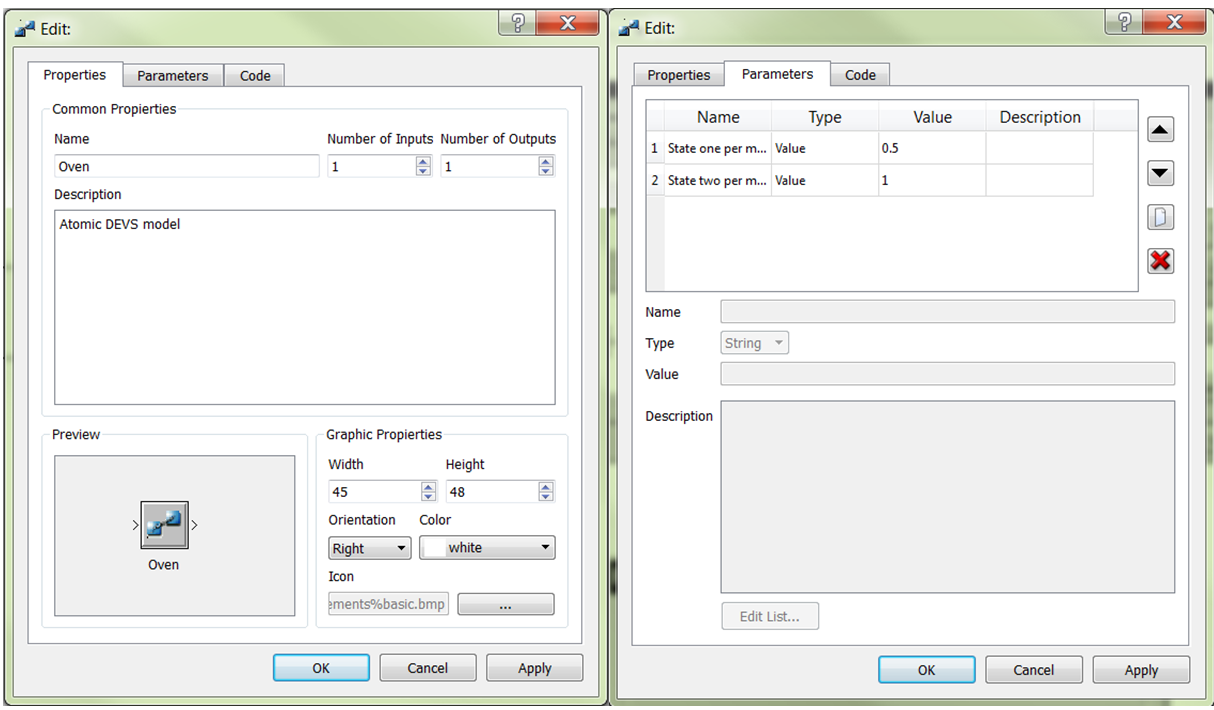
\includegraphics[width=0.85\textwidth]{Fig4.png}
    \caption{Block Edition Window}
    \label{Block_win}
\end{figure}

The Coupled models have no an associated code and there are some other extra features which can be modified in block edition window and the edit menu. Various input and output ports of a coupled model are characterized by their names. The order of their appearance in the block can be changed in the edition window. Priorities can be established in edition menu of corresponding model to solve the simultaneous occurrence of event among blocks at the same sub–model.

\begin{figure}[h!]
  \centering
    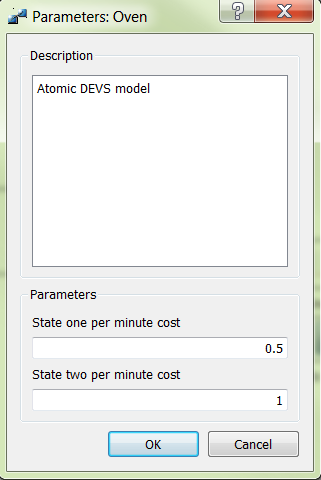
\includegraphics[width=0.5\textwidth]{Fig5.png}
    \caption{Parameter changing window}
    \label{para_win}
\end{figure}


\subsubsection{The Atomic Editor}
The Atomic Editor facilitates the edition of C++ code corresponding to each DEVS model. The transition functions, output function, time advance, etc. for DEVS atomic models of elementary blocks are defined in it.


\begin{figure}[h!]
  \centering
    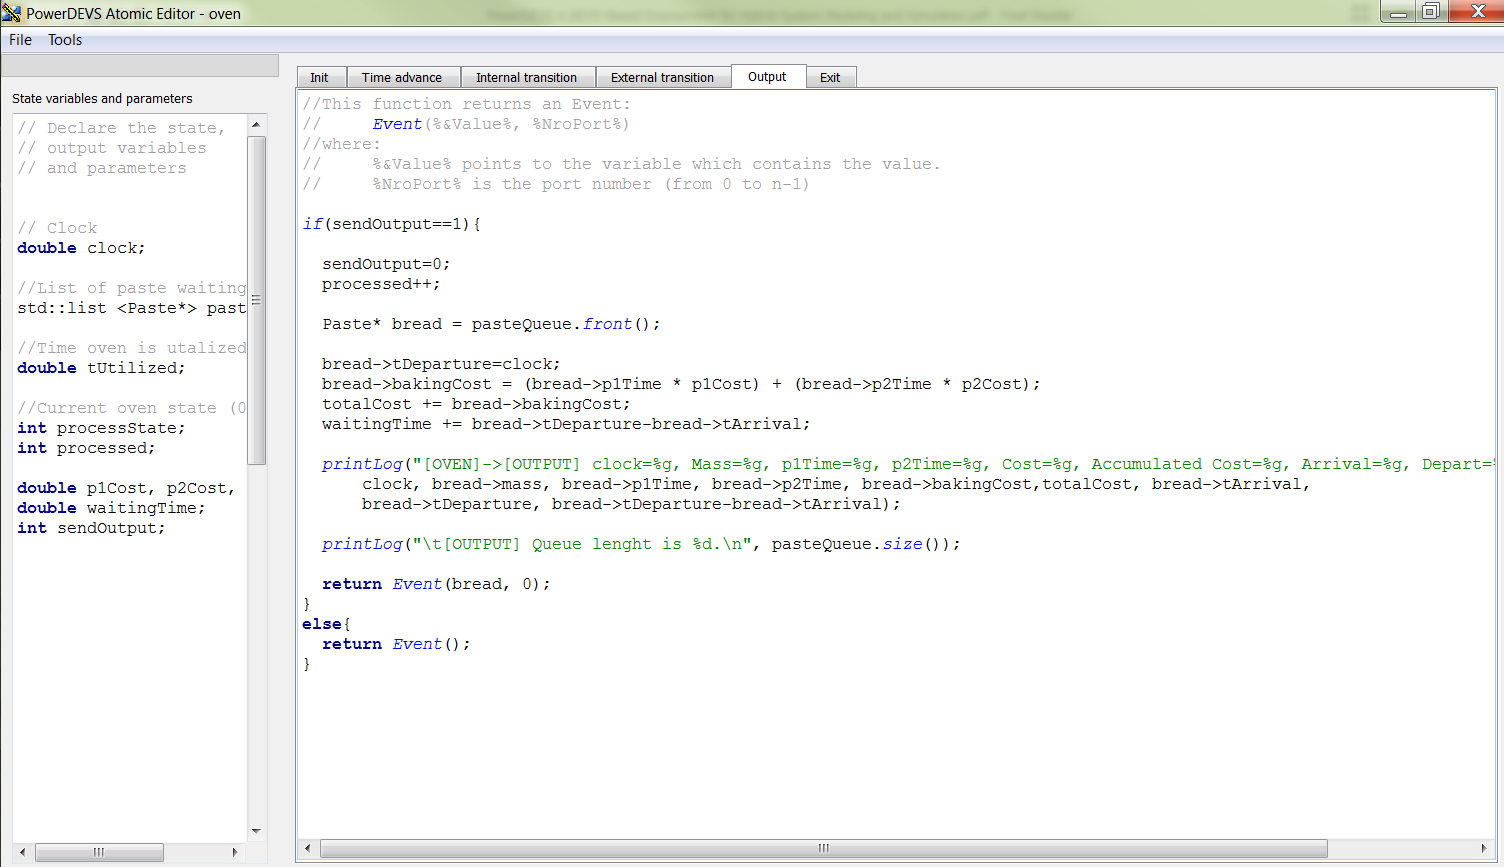
\includegraphics[width=0.9\textwidth]{Fig6.png}
    \caption{Atomic Editor main window}
    \label{atomic_win}
\end{figure}

It can be invoked from the Edition Window to edit an existing code or to create a new one. It can be also run directly from Windows since it is a standalone application. The Atomic Editor main window is shown in Figure \ref{atomic_win}. In atomic editor the state variables, the output of the DEVS model and the variables of system parameters are only defined. Then the C++ code for time advance, transition and output functions has to be placed in the corresponding windows and when the model is saved, the code is automatically completed and stored in the corresponding .cpp and .h files. The Atomic Editor was also designed to write a code which is very similar to the DEVS model definition. All the rest of the job related to simulation and implementation topics is automatically performed by the program.
\subsubsection{Structure Generator}
A PowerDEVS model is defined by block diagram in dot pdm file which represent system structure and the atomic models in dot h and dot cpp files which are generated by the atomic editor. Then, the simulation is run using Quick Simulation command in the Simulation menu of the Model Editor. The Quick Simulation command performs the simulation and PowerDEVS model is converted into a standalone program that executes the simulation. The final simulation time is only asked in this command and then the simulation is executed.
The conversion of the model into a simulation program is done in two steps. The Structure Generator converts the model file (.pdm) which contains all the information about the model, into a coupled DEVS specification. The Structure Generator produces a dot pds file which only contains the information about connections, location of atomic models and block parameters, etc., needed to build the simulation file. The coupling specification of the model is also converted into a formal DEVS coupling specification. As the Structure Generator is a standalone program so it can be run directly from the Simulation menu or from the command line. If it is run in that way, it produces a report in dot pds file showing the output. Figure \ref{Struc_gen} shows the out of structure generator.


\begin{figure}[h!]
  \centering
    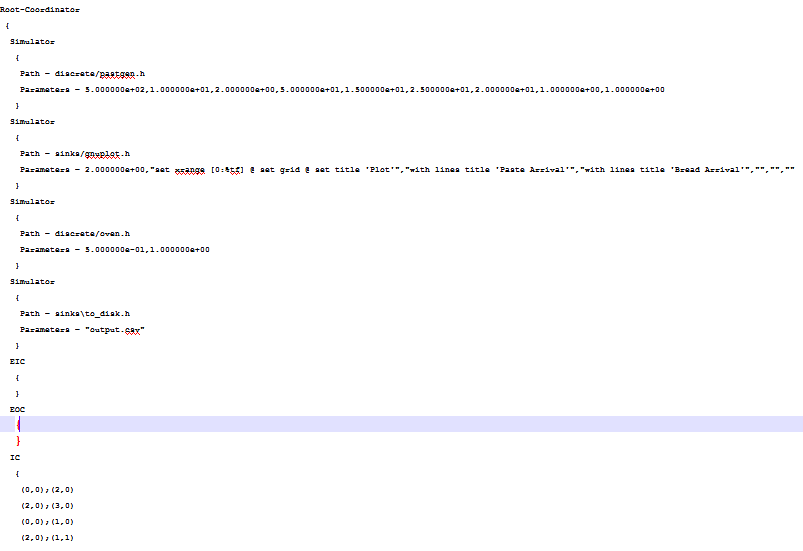
\includegraphics[width=0.9\textwidth]{Fig7.png}
    \caption{Structure Generator output}
    \label{Struc_gen}
\end{figure}



\subsubsection{The Preprocessor}
The Preprocessor translates the model editor files into structure files which contain the coupling structure and the information to build up the simulation code, links the code of the different atomic models according to the corresponding structure file and compiles it to produce a standalone executable file which simulates the system. It basically translates the \texttt{.pds} file into a header dot h file which binds the simulators and coordinators according to the coupling structure. The preprocessor also produces a make file which is then invoked to generate the program which executes the simulation. The Preprocessor can be invoked in a transparent way using the Quick Simulation command.

\subsubsection{The Simulation Interface }
The Simulation Interface ( Figure \ref{sim_int} ) runs the stand alone executable files according to the structure of PowerDEVS as shown in Figure \ref{sim_st} and provides to change the parameters of simulation like final time, number of simulations to perform, and the simulation mode (normal simulation, timed simulation, step-by-step simulation, etc.).


\begin{figure}[h!]
  \centering
    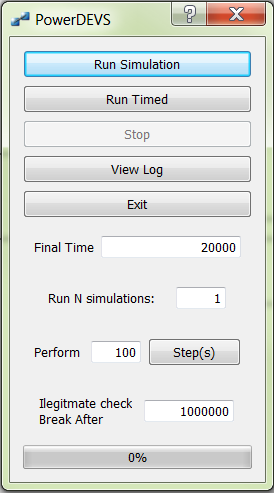
\includegraphics[width=0.5\textwidth]{Fig8.png}
    \caption{Simulation interface}
    \label{sim_int}
\end{figure}


\begin{figure}[h!]
  \centering
    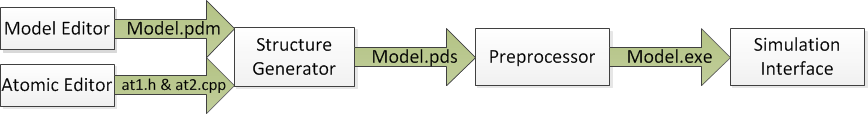
\includegraphics[width=0.7\textwidth]{Fig9.png}
    \caption{Simulation structure of PowerDEVS}
    \label{sim_st}
\end{figure}


 
\subsubsection{A running instance of Scilab}

It acts as a workspace, where the simulation parameters can be read and results can be exported to. This instance is a modification of Scilab 4.1.2 to support this type of operations as shown in Figure \ref{sci_in}.




\begin{figure}[h!]
  \centering
    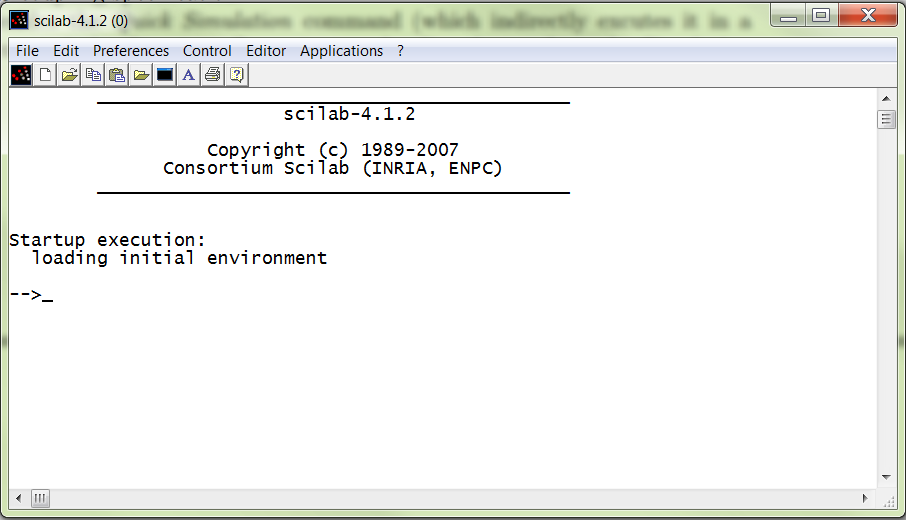
\includegraphics[width=0.7\textwidth]{Fig10.png}
    \caption{Scilab Instance}
    \label{sci_in}
\end{figure}

All the applications of \pd except Model Editor were programmed in C++ with the graphical libraries QT and Model Editor was only application programmed in Visual Basic. PowerDEVS can runs under a real time operating system (\cite{ManRTI}) synchronizing the event with a real–time clock with the capability of capturing interrupts at the atomic level. PowerDEVS also allows the direct implementation of asynchronous DEVS–based Quantized State Controllers \cite{Kof03b} on a PC.




\subsection{Power DEVS implementation Details}
\subsection{Most challenging subtask of the project}




\section{Task 4 : Simulation Results}
%========================================Bibliography=====================================
\bibliographystyle{plain}


\bibliography{ref}

%========================================Appendix=====================================

\newpage
\appendix

\section{Code Listings}

\subsection{UC 1}





\end{document}
